\section{Results}
\label{sec:results}

Table~\ref{tab:main} summarises the main experiment and Figure~\ref{fig:length} shows the headline result. Unless stated otherwise, numbers are means over 10 seeds with 95\% $t$-intervals, evaluated with the checkpoint selected on training-length validation. Paired differences give the mean difference over seeds, its interval, the number of seeds favouring the first method, and a sign-flip $p$-value.

\begin{figure}[t]
\centering
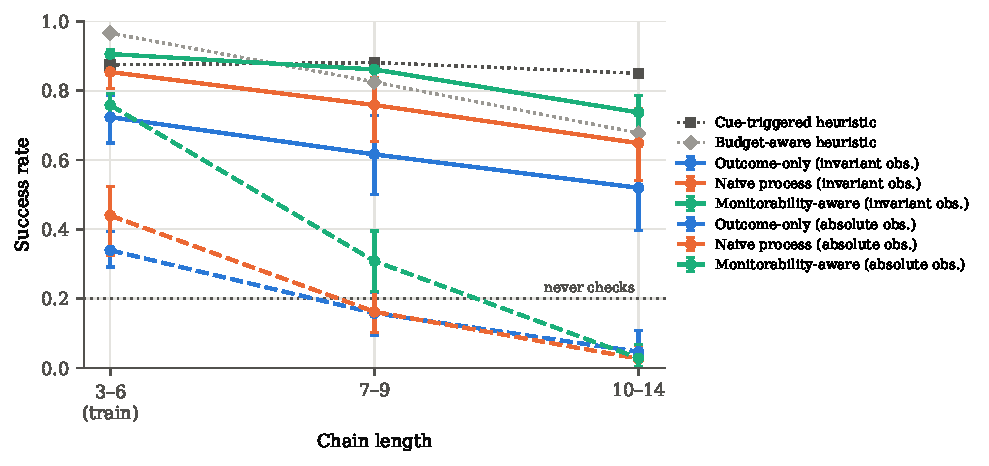
\includegraphics[width=0.92\linewidth]{figures/length_generalization.pdf}
\caption{Success on training lengths (3--6) and on longer held-out chains. Colour encodes the reward and line style the observation encoder (solid: invariant, dashed: absolute); error bars are 95\% $t$-intervals over 10 seeds. With absolute features every reward scheme drops below a policy that never checks. With invariant features the monitorability-aware agent comes within a few points of the cue-triggered heuristic at lengths 7--9.}
\label{fig:length}
\end{figure}

\begin{table}[t]
\centering
\small
\setlength{\tabcolsep}{3.5pt}
\caption{Main results (mean over 10 seeds, 95\% $t$-interval). ``Detect'' is the fraction of faulty episodes in which a check caught the fault; ``cost-adj.'' is success minus $0.05\times$ budget spent. Top block: hand-coded references; bottom block: learned agents (checkpoint selected on training lengths only).}
\label{tab:main}
\resizebox{\linewidth}{!}{\begin{tabular}{lccccc}
\toprule
Method & Success 3--6 & Success 7--9 & Success 10--14 & Detect 7--9 & Cost-adj. 7--9 \\
\midrule
Random & 0.00\,{\scriptsize[0.00, 0.01]} & 0.00\,{\scriptsize[0.00, 0.00]} & 0.00\,{\scriptsize[0.00, 0.00]} & 0.02\,{\scriptsize[0.01, 0.02]} & -0.09\,{\scriptsize[-0.09, -0.08]} \\
Always THINK & 0.20\,{\scriptsize[0.19, 0.21]} & 0.20\,{\scriptsize[0.19, 0.21]} & 0.20\,{\scriptsize[0.19, 0.21]} & 0.00\,{\scriptsize[0.00, 0.00]} & -0.20\,{\scriptsize[-0.21, -0.19]} \\
Verify every step & 0.80\,{\scriptsize[0.79, 0.81]} & 0.06\,{\scriptsize[0.06, 0.07]} & 0.00\,{\scriptsize[0.00, 0.00]} & 0.93\,{\scriptsize[0.92, 0.94]} & -0.63\,{\scriptsize[-0.64, -0.63]} \\
Cue-triggered & 0.87\,{\scriptsize[0.87, 0.88]} & 0.88\,{\scriptsize[0.87, 0.89]} & 0.85\,{\scriptsize[0.84, 0.86]} & 0.85\,{\scriptsize[0.84, 0.87]} & 0.33\,{\scriptsize[0.31, 0.34]} \\
Budget-aware & 0.97\,{\scriptsize[0.96, 0.97]} & 0.82\,{\scriptsize[0.81, 0.84]} & 0.68\,{\scriptsize[0.66, 0.70]} & 0.78\,{\scriptsize[0.76, 0.79]} & 0.19\,{\scriptsize[0.17, 0.20]} \\
\midrule
Outcome (inv) & 0.72\,{\scriptsize[0.65, 0.79]} & 0.62\,{\scriptsize[0.50, 0.73]} & 0.52\,{\scriptsize[0.40, 0.65]} & 0.61\,{\scriptsize[0.45, 0.75]} & -0.02\,{\scriptsize[-0.14, 0.09]} \\
Naive process (inv) & 0.85\,{\scriptsize[0.81, 0.89]} & 0.76\,{\scriptsize[0.65, 0.84]} & 0.65\,{\scriptsize[0.54, 0.75]} & 0.76\,{\scriptsize[0.63, 0.86]} & 0.09\,{\scriptsize[-0.01, 0.18]} \\
Monitorability (inv) & 0.91\,{\scriptsize[0.89, 0.92]} & 0.86\,{\scriptsize[0.84, 0.89]} & 0.74\,{\scriptsize[0.69, 0.79]} & 0.85\,{\scriptsize[0.83, 0.87]} & 0.19\,{\scriptsize[0.15, 0.22]} \\
Outcome (abs) & 0.34\,{\scriptsize[0.29, 0.39]} & 0.16\,{\scriptsize[0.09, 0.22]} & 0.05\,{\scriptsize[0.00, 0.11]} & 0.09\,{\scriptsize[0.04, 0.16]} & -0.27\,{\scriptsize[-0.36, -0.17]} \\
Naive process (abs) & 0.44\,{\scriptsize[0.33, 0.52]} & 0.16\,{\scriptsize[0.10, 0.22]} & 0.03\,{\scriptsize[0.00, 0.06]} & 0.30\,{\scriptsize[0.14, 0.49]} & -0.32\,{\scriptsize[-0.42, -0.23]} \\
Monitorability (abs) & 0.76\,{\scriptsize[0.73, 0.79]} & 0.31\,{\scriptsize[0.22, 0.39]} & 0.03\,{\scriptsize[0.00, 0.07]} & 0.60\,{\scriptsize[0.46, 0.72]} & -0.24\,{\scriptsize[-0.32, -0.18]} \\
\bottomrule
\end{tabular}
}
\end{table}

\subsection{Process rewards make checking learnable and reduce collapse}
\label{sec:learnability}

Never checking succeeds exactly when no fault is present, which happens 20\% of the time. Any gain above that requires the agent to discover a three-step pattern: check a suspicious step, see \textsc{unsafe}, then undo and redo.

\paragraph{Absolute observations.}
Outcome-only agents essentially never acquire this pattern. In \val{main/outcome_abs/seeds_peak_above_half}/10 seeds does any validation checkpoint exceed 0.5 success, and the selected checkpoints reach \ci{main/outcome_abs/train_like/success} on training lengths. The monitorability-aware reward reaches \ci{main/ma_abs/train_like/success} (paired $+$\val{diff/ma_abs-outcome_abs/train_like/success} [\val{diff/ma_abs-outcome_abs/train_like/success/lo}, \val{diff/ma_abs-outcome_abs/train_like/success/hi}], \val{diff/ma_abs-outcome_abs/train_like/success/npos}/10 seeds, $p=\val{diff/ma_abs-outcome_abs/train_like/success/p}$).

\paragraph{Invariant observations.}
Outcome-only agents \emph{do} find checking policies: some validation checkpoint exceeds 0.5 in \val{main/outcome_inv/seeds_peak_above_half}/10 seeds. They rarely keep them. After the first 5{,}000 episodes, \val{main/outcome_inv/collapse_nevercheck_rate/pct} of their greedy checkpoints have stopped checking altogether (success $\le 0.35$ and fault detection below 0.2; Figure~\ref{fig:curves}). Under the monitorability-aware reward \val{main/ma_inv/collapse_nevercheck_rate/pct} of late checkpoints have. At selected checkpoints, the monitorability-aware reward beats outcome-only by $+$\val{diff/ma_inv-outcome_inv/train_like/success} [\val{diff/ma_inv-outcome_inv/train_like/success/lo}, \val{diff/ma_inv-outcome_inv/train_like/success/hi}] ($p=\val{diff/ma_inv-outcome_inv/train_like/success/p}$). Its advantage over naive process reward is smaller and less certain: $+$\val{diff/ma_inv-naive_inv/train_like/success} [\val{diff/ma_inv-naive_inv/train_like/success/lo}, \val{diff/ma_inv-naive_inv/train_like/success/hi}], \val{diff/ma_inv-naive_inv/train_like/success/npos}/10 seeds, $p=\val{diff/ma_inv-naive_inv/train_like/success/p}$. Its training-length success of \ci{main/ma_inv/train_like/success} lies between the cue-triggered heuristic (\val{main/cue_triggered/train_like/success}) and the tuned budget-aware heuristic (\val{main/budget_aware_1/train_like/success}).

\begin{figure}[t]
\centering
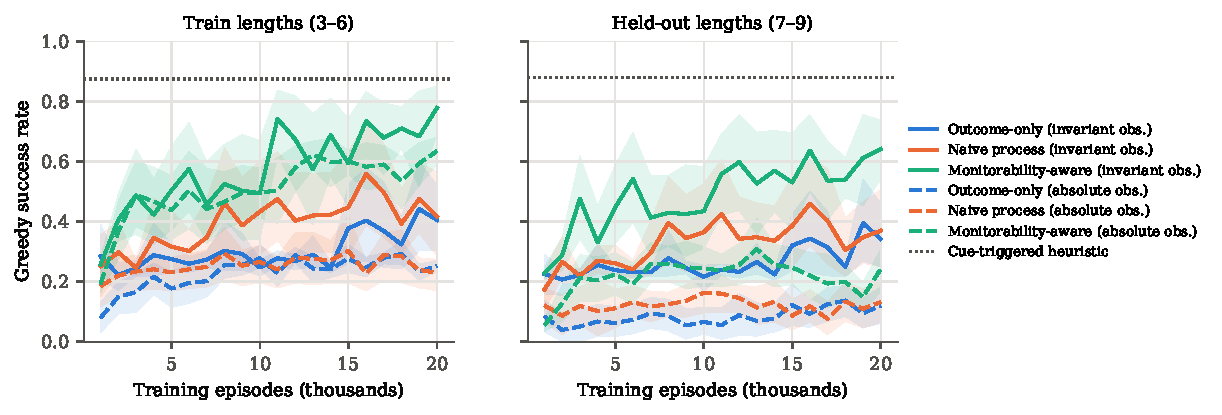
\includegraphics[width=\linewidth]{figures/learning_curves.pdf}
\caption{Greedy success during training (mean over 10 seeds, shaded 95\% $t$-interval), evaluated every 1{,}000 episodes on validation episodes. The mean hides large per-seed swings (Figure~\ref{fig:churn}).}
\label{fig:curves}
\end{figure}

\subsection{A side effect of the reward: detecting without repairing}
\label{sec:norepair}

The monitorability-aware agents' low-success checkpoints are not never-check policies. Of the late checkpoints of the invariant agent, \val{main/ma_inv/collapse_rate/pct} have success $\le 0.35$. Of these, \val{main/ma_inv/collapse_norepair_rate/pct} of all late checkpoints still catch at least half of all faults, but fail to complete the repair. This is what the reward pays for. The $0.25$ fault bonus, plus $0.18$ if the step was cued, is earned when the fault is caught, whether or not the agent then undoes and redoes the step. The effect is visible in the evaluated agents too (Appendix Table~\ref{tab:behaviour}). Even on training lengths, where no input is out of range, the last checkpoints complete the repair after a caught fault in only \val{main/ma_abs@final/train_like/success_given_detected/pct} (absolute features) and \val{main/ma_inv@final/train_like/success_given_detected/pct} (invariant features) of episodes, against \val{main/cue_triggered/train_like/success_given_detected/pct} for the hand-coded policies. Moving the fault bonus from detection to repair is a direct test of this explanation (\S\ref{sec:followups}).

\subsection{Length generalization is mainly a representation problem}
\label{sec:length}

Figure~\ref{fig:length} separates the effect of the reward from the effect of the observation encoding. With absolute features, success falls sharply on longer chains for every reward. On lengths 10--14 all three absolute-feature agents are \emph{worse than never checking}: \val{main/outcome_abs/heldout_xlong/success}, \val{main/naive_abs/heldout_xlong/success} and \val{main/ma_abs/heldout_xlong/success}, versus \val{main/always_think/heldout_xlong/success}.

The explanation is that every observation the absolute encoder produces on held-out lengths is new: across rollouts of the hand-coded policies, \val{coverage/absolute/heldout_long/unseen_rate/pct} of decision points at lengths 7--9 have an observation vector that never occurs at lengths 3--6. For the invariant encoder the figure is \val{coverage/invariant/heldout_long/unseen_rate/pct} at 7--9 and \val{coverage/invariant/heldout_xlong/unseen_rate/pct} at 10--14. The absolute-feature policies act erratically on these inputs. For example, on lengths 10--14, \val{main/ma_abs/heldout_xlong/voluntary_incomplete_commit/pct} of monitorability-aware episodes end with a \texttt{COMMIT} before the chain is finished although the remaining budget could still finish it.

Changing only the observation encoder removes most of the failure. The monitorability-aware agent with invariant features keeps \ci{main/ma_inv/heldout_long/success} at lengths 7--9 and \ci{main/ma_inv/heldout_xlong/success} at 10--14. These are paired improvements over the absolute encoder of $+$\val{diff/ma_inv-ma_abs/heldout_long/success} [\val{diff/ma_inv-ma_abs/heldout_long/success/lo}, \val{diff/ma_inv-ma_abs/heldout_long/success/hi}] and $+$\val{diff/ma_inv-ma_abs/heldout_xlong/success} [\val{diff/ma_inv-ma_abs/heldout_xlong/success/lo}, \val{diff/ma_inv-ma_abs/heldout_xlong/success/hi}], in \val{diff/ma_inv-ma_abs/heldout_xlong/success/npos}/10 seeds ($p=\val{diff/ma_inv-ma_abs/heldout_xlong/success/p}$). At lengths 7--9 the agent comes within \val{diff/ma_inv-cue_triggered/heldout_long/success} [\val{diff/ma_inv-cue_triggered/heldout_long/success/lo}, \val{diff/ma_inv-cue_triggered/heldout_long/success/hi}] of the cue-triggered heuristic. This is not a significant difference ($p=\val{diff/ma_inv-cue_triggered/heldout_long/success/p}$), but it is not a demonstration of equivalence either.

The reward still matters under the invariant encoder. The monitorability-aware reward beats outcome-only at every length ($+$\val{diff/ma_inv-outcome_inv/heldout_long/success}, $p=\val{diff/ma_inv-outcome_inv/heldout_long/success/p}$ at 7--9; $+$\val{diff/ma_inv-outcome_inv/heldout_xlong/success}, $p=\val{diff/ma_inv-outcome_inv/heldout_xlong/success/p}$ at 10--14). Naive process reward falls between the two in point estimate, but with 10 seeds its separation from either neighbour is not resolved on held-out lengths (for example, monitorability-aware minus naive at 10--14: $+$\val{diff/ma_inv-naive_inv/heldout_xlong/success} [\val{diff/ma_inv-naive_inv/heldout_xlong/success/lo}, \val{diff/ma_inv-naive_inv/heldout_xlong/success/hi}]).

\subsection{What the agents learn: checking cued steps}
\label{sec:selectivity}

Figure~\ref{fig:selectivity} shows how often each agent checks at a decision point whose current step is unchecked, split by whether that step's cue fired. With invariant features all three rewards produce cue-conditional checking. What distinguishes the monitorability-aware reward is \emph{coverage} of cued steps, not avoidance of un-cued ones. It checks at \val{main/ma_inv/train_like/verify_rate_cue1} of cued decision points versus \val{main/outcome_inv/train_like/verify_rate_cue1} for outcome-only, while checking un-cued ones at a similar rate (\val{main/ma_inv/train_like/verify_rate_cue0} vs.\ \val{main/outcome_inv/train_like/verify_rate_cue0}). Outcome-only agents with absolute features barely condition on the cue at all (\val{main/outcome_abs/train_like/verify_rate_cue1} vs.\ \val{main/outcome_abs/train_like/verify_rate_cue0}). With absolute features, the monitorability-aware agent's cue coverage decays on held-out lengths (\val{main/ma_abs/heldout_long/verify_rate_cue1} at 7--9). With invariant features it is largely preserved (\val{main/ma_inv/heldout_long/verify_rate_cue1}).

\begin{figure}[t]
\centering
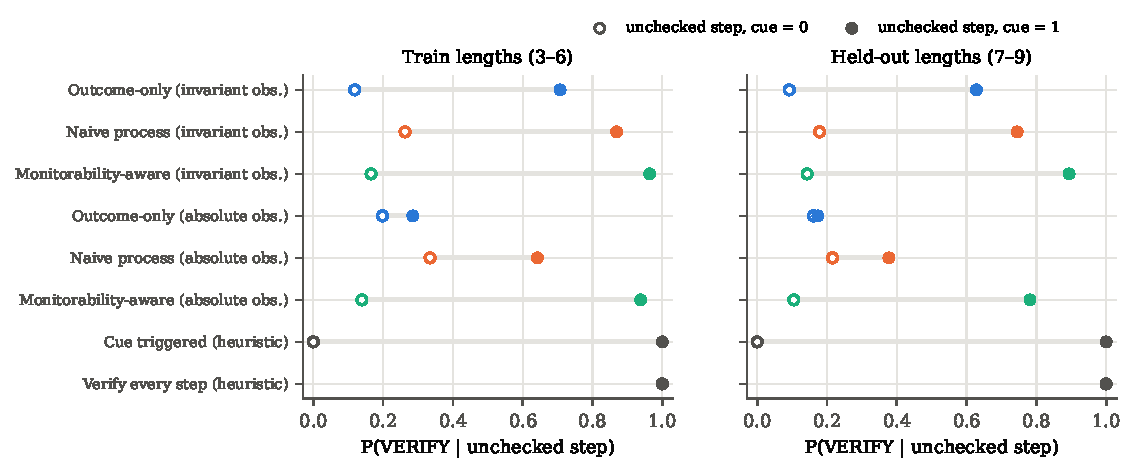
\includegraphics[width=\linewidth]{figures/cue_selectivity.pdf}
\caption{Cue-conditional checking: probability of choosing \texttt{VERIFY} at a decision point whose current step is unchecked, when that step's cue is off (open) or on (filled). The cue-triggered heuristic is perfectly cue-conditional by construction.}
\label{fig:selectivity}
\end{figure}

\subsection{The residual gap: spending slack that long chains need}
\label{sec:residual}

The invariant agents still lose ground on the longest chains (\val{main/ma_inv/train_like/success} $\to$ \val{main/ma_inv/heldout_long/success} $\to$ \val{main/ma_inv/heldout_xlong/success}). The cue-triggered heuristic does not (\val{main/cue_triggered/train_like/success} $\to$ \val{main/cue_triggered/heldout_long/success} $\to$ \val{main/cue_triggered/heldout_xlong/success}). The budget-aware heuristic, tuned on training lengths, degrades like the learned agent (\val{main/budget_aware_1/train_like/success} $\to$ \val{main/budget_aware_1/heldout_long/success} $\to$ \val{main/budget_aware_1/heldout_xlong/success}), which points to how the budget is allocated rather than to the representation. The six units of slack beyond the chain length must cover every cued check plus one repair.
\begin{itemize}
  \item \textbf{Un-cued checks.} On short chains, slack is left over for checking un-cued steps, which pays off. On long chains there are more cued steps to cover, and slack spent early is missing later.
  \item \textbf{Non-repair \texttt{REVISE}s.} The learned agents also spend slack on \texttt{REVISE}s that cannot be repairs (\val{main/ma_inv/heldout_xlong/nonrepair_revise_count} per episode at 10--14, each costing two units with its re-execution). This is a consequence of the memoryless observation (\S\ref{sec:setup}): after a \textsc{safe} check, undoing and redoing a step leads to the same observation as a genuine repair.
\end{itemize}
Both effects reduce fault detection at 10--14 to \val{main/ma_inv/heldout_xlong/fault_detected} for the learned agent and \val{main/budget_aware_1/heldout_xlong/fault_detected} for the budget-aware heuristic, against \val{main/cue_triggered/heldout_xlong/fault_detected} for the cue-triggered one. The best allocation genuinely depends on how many steps remain, which the invariant encoder hides. \S\ref{sec:followups} tests a memory bit and a remaining-length feature.

\subsection{Robustness to environment shifts}
\label{sec:shifts}

Table~\ref{tab:shifts} evaluates policies at lengths 7--9 under shifts they were not trained on.
\begin{itemize}
  \item \textbf{Fault rate.} The invariant monitorability-aware agent is robust to the fault rate (\val{main/ma_inv/fault_0.6/success} at $p_f{=}0.6$, \val{main/ma_inv/fault_0.9/success} at $p_f{=}0.9$).
  \item \textbf{Cue quality.} It tracks the cue-triggered heuristic when cue quality changes (clean: \val{main/ma_inv/cue_clean/success} vs.\ \val{main/cue_triggered/cue_clean/success}; noisy: \val{main/ma_inv/cue_noisy/success} vs.\ \val{main/cue_triggered/cue_noisy/success}). This confirms that the policy relies on the cue rather than on a fixed checking schedule.
  \item \textbf{Verification cost.} It degrades when checks cost more than in training (\val{main/ma_inv/verify_cost_3/success} at $c_V{=}3$), because it keeps checking at a rate the budget no longer supports.
  \item \textbf{Budget slack.} It is sensitive to the slack in \emph{both} directions. With slack 4, success falls to \val{main/ma_inv/budget_extra_4/success} (cue-triggered: \val{main/cue_triggered/budget_extra_4/success}), although every slack value then stays inside the training range. This is the allocation problem of \S\ref{sec:residual} again: a checking rate tuned to slack 6 runs out of budget. With slack 8, success falls to \val{main/ma_inv/budget_extra_8/success}. Here the budget-aware heuristic improves (\val{main/budget_aware_1/budget_extra_8/success}), and the cue-triggered heuristic, which never spends extra slack, is unchanged (\val{main/cue_triggered/budget_extra_8/success}). With slack 8 the slack feature also takes values never seen in training. The ``invariant'' encoder is invariant to length, not to budget.
\end{itemize}

\begin{table}[t]
\centering
\small
\setlength{\tabcolsep}{3pt}
\caption{Success under shifts at held-out lengths 7--9, without retraining (mean over 10 seeds). $p_f$: fault probability (train: 0.8); $c_V$: verification cost (train: 1); slack: extra budget beyond the chain length (train: 6); clean/noisy cue: hit/false-positive rates $0.95/0.05$ and $0.60/0.35$ (train: $0.85/0.15$).}
\label{tab:shifts}
\resizebox{\linewidth}{!}{\begin{tabular}{lccccccccc}
\toprule
Method & default & $p_f{=}0.6$ & $p_f{=}0.9$ & $c_V{=}2$ & $c_V{=}3$ & slack 4 & slack 8 & clean cue & noisy cue \\
\midrule
Always THINK & 0.20 & 0.41 & 0.10 & 0.20 & 0.19 & 0.20 & 0.21 & 0.21 & 0.20 \\
Cue-triggered & 0.88 & 0.91 & 0.86 & 0.75 & 0.49 & 0.73 & 0.88 & 0.96 & 0.62 \\
Budget-aware & 0.82 & 0.88 & 0.81 & 0.66 & 0.22 & 0.67 & 0.95 & 0.93 & 0.65 \\
Outcome (inv) & 0.62 & 0.72 & 0.56 & 0.51 & 0.22 & 0.42 & 0.41 & 0.75 & 0.41 \\
Naive process (inv) & 0.76 & 0.83 & 0.74 & 0.56 & 0.26 & 0.44 & 0.68 & 0.87 & 0.55 \\
Monitorability (abs) & 0.31 & 0.41 & 0.27 & 0.25 & 0.11 & 0.23 & 0.36 & 0.37 & 0.22 \\
Monitorability (inv) & 0.86 & 0.90 & 0.85 & 0.69 & 0.24 & 0.49 & 0.65 & 0.94 & 0.64 \\
\bottomrule
\end{tabular}
}
\end{table}

\subsection{Which reward terms matter}
\label{sec:ablations}

Table~\ref{tab:ablations} removes one group of terms at a time from the monitorability-aware reward, with invariant observations and 10 seeds each. Because every variant is evaluated on the same episodes as the full reward, the differences below are paired.
\begin{itemize}
  \item \textbf{Cue terms.} The cue terms (the bonus for informative checks of cued steps and the small penalty for checking un-cued ones) are the only component whose removal substantially hurts generalization. Without them, held-out success drops by \val{abl/ma_inv-no_cue_terms/heldout_long/success} [\val{abl/ma_inv-no_cue_terms/heldout_long/success/lo}, \val{abl/ma_inv-no_cue_terms/heldout_long/success/hi}] at lengths 7--9 and by \val{abl/ma_inv-no_cue_terms/heldout_xlong/success} [\val{abl/ma_inv-no_cue_terms/heldout_xlong/success/lo}, \val{abl/ma_inv-no_cue_terms/heldout_xlong/success/hi}] at 10--14 ($p = \val{abl/ma_inv-no_cue_terms/heldout_xlong/success/p}$), while training-length success barely changes (\val{ablations/no_cue_terms/train_like/success} vs.\ \val{ablations/ma_inv/train_like/success}). The mechanism is visible in the checking rates. Without the cue terms, agents check un-cued steps at about twice the rate (\val{ablations/no_cue_terms/heldout_long/verify_rate_cue0} vs.\ \val{ablations/ma_inv/heldout_long/verify_rate_cue0} at 7--9). That costs little on short chains, but spends the slack that long chains need.
  \item \textbf{Cue bonus alone.} Conversely, the cue bonus alone, with every other process term removed, is indistinguishable from the full reward (\val{ablations/cue_bonus_only/heldout_long/success} at 7--9 and \val{ablations/cue_bonus_only/heldout_xlong/success} at 10--14, vs.\ \val{ablations/ma_inv/heldout_long/success} and \val{ablations/ma_inv/heldout_xlong/success}).
  \item \textbf{Other terms.} Removing the unchecked-gap term or the wasted-check penalty has no resolvable effect. Removing the safe/fault check bonuses, or all of the cue, gap and waste terms together, lowers held-out success moderately. Removing the per-action cost hurts at every length.
  \item \textbf{No \texttt{REVISE}.} Without \texttt{REVISE}, a caught fault cannot be repaired and success falls to the never-check level (\val{ablations/no_revise/train_like/success}).
\end{itemize}
In short, most of what the monitorability-aware reward contributes in this environment comes from one term: paying for checks where a trusted cue says checking is valuable.

\begin{table}[t]
\centering
\small
\setlength{\tabcolsep}{3pt}
\caption{Reward ablations (invariant observations; mean over 10 seeds, 95\% $t$-interval). $P(V \mid c)$: probability of checking at a decision point whose current step is unchecked with cue $c$, at lengths 7--9.}
\label{tab:ablations}
\resizebox{\linewidth}{!}{\begin{tabular}{lccccc}
\toprule
Variant & Success 3--6 & Success 7--9 & Success 10--14 & $P(V\mid c{=}1)$ & $P(V\mid c{=}0)$ \\
\midrule
Full reward & 0.91\,{\scriptsize[0.89, 0.92]} & 0.86\,{\scriptsize[0.84, 0.89]} & 0.74\,{\scriptsize[0.69, 0.79]} & 0.89 & 0.14 \\
$-$ cue bonus/penalty & 0.88\,{\scriptsize[0.85, 0.90]} & 0.64\,{\scriptsize[0.58, 0.71]} & 0.40\,{\scriptsize[0.33, 0.50]} & 0.83 & 0.30 \\
$-$ unchecked-gap term & 0.89\,{\scriptsize[0.87, 0.91]} & 0.84\,{\scriptsize[0.81, 0.86]} & 0.73\,{\scriptsize[0.62, 0.82]} & 0.88 & 0.13 \\
$-$ wasted-check penalty & 0.89\,{\scriptsize[0.87, 0.91]} & 0.85\,{\scriptsize[0.81, 0.88]} & 0.68\,{\scriptsize[0.54, 0.78]} & 0.92 & 0.15 \\
$-$ safe/fault check bonuses & 0.89\,{\scriptsize[0.88, 0.89]} & 0.78\,{\scriptsize[0.75, 0.81]} & 0.65\,{\scriptsize[0.57, 0.72]} & 0.92 & 0.15 \\
$-$ cue, gap and waste terms & 0.89\,{\scriptsize[0.88, 0.90]} & 0.79\,{\scriptsize[0.73, 0.83]} & 0.66\,{\scriptsize[0.57, 0.73]} & 0.83 & 0.16 \\
cue bonus only & 0.88\,{\scriptsize[0.87, 0.90]} & 0.85\,{\scriptsize[0.83, 0.87]} & 0.77\,{\scriptsize[0.73, 0.82]} & 0.92 & 0.10 \\
$-$ per-action cost & 0.85\,{\scriptsize[0.81, 0.88]} & 0.76\,{\scriptsize[0.70, 0.81]} & 0.61\,{\scriptsize[0.52, 0.69]} & 0.92 & 0.11 \\
REVISE disabled & 0.20\,{\scriptsize[0.19, 0.21]} & 0.19\,{\scriptsize[0.17, 0.20]} & 0.15\,{\scriptsize[0.13, 0.18]} & 0.61 & 0.11 \\
\bottomrule
\end{tabular}
}
\end{table}


\subsection{Training stability and sensitivity}
\label{sec:stability}
\label{sec:sensitivity}

DQN agents in this environment exhibit severe policy churn~\citep{schaul2022churn}. Figure~\ref{fig:churn} plots greedy success for each seed of the two monitorability-aware conditions. Policies repeatedly switch, within a few thousand episodes, between a solution that checks and repairs ($\approx$0.9) and one that checks but does not repair ($\approx$0.25--0.3; \S\ref{sec:norepair}). After the first 5{,}000 episodes, the mean absolute change in training-length success between consecutive evaluations is \val{main/ma_inv/mean_abs_change} for the invariant monitorability-aware agent. That is larger than for outcome-only agents (\val{main/outcome_inv/mean_abs_change}), which mostly sit in the never-check regime.

Because of this churn, last-checkpoint results (Appendix Table~\ref{tab:final}) are lower and noisier than selected-checkpoint results. For example, the invariant monitorability-aware agent scores \ci{main/ma_inv@final/heldout_long/success} instead of \ci{main/ma_inv/heldout_long/success} at lengths 7--9. With last checkpoints, the results split three ways:
\begin{itemize}
  \item \textbf{Unchanged:} the encoder gap ($+$\val{diff/ma_inv@final-ma_abs@final/heldout_xlong/success} at 10--14, $p=\val{diff/ma_inv@final-ma_abs@final/heldout_xlong/success/p}$) and the advantage of the monitorability-aware reward over outcome-only ($+$\val{diff/ma_inv@final-outcome_inv@final/heldout_long/success} at 7--9, $p=\val{diff/ma_inv@final-outcome_inv@final/heldout_long/success/p}$).
  \item \textbf{Weakened:} naive process reward is no longer separable from outcome-only ($+$\val{diff/naive_inv@final-outcome_inv@final/heldout_long/success} [\val{diff/naive_inv@final-outcome_inv@final/heldout_long/success/lo}, \val{diff/naive_inv@final-outcome_inv@final/heldout_long/success/hi}]).
  \item \textbf{Lost:} closeness to the cue-triggered heuristic. The last checkpoint is \val{diff/ma_inv@final-cue_triggered/heldout_long/success} [\val{diff/ma_inv@final-cue_triggered/heldout_long/success/lo}, \val{diff/ma_inv@final-cue_triggered/heldout_long/success/hi}] below it at lengths 7--9.
\end{itemize}
Selection uses only training-length validation episodes, so it cannot favour the encoder that generalizes better.

The main experiment uses the earlier version's DQN settings. To check that the encoder effect and the reward comparison are not specific to them, we retrain the monitorability-aware agents with both encoders, and outcome-only and naive agents with the invariant encoder, under three alternatives, five seeds each: learning rate $3{\cdot}10^{-4}$; hard target updates every 1{,}000 steps; and Polyak-averaged targets ($\tau = 0.005$)~\citep{lillicrap2016continuous} (Table~\ref{tab:sensitivity}). None of them removes the churn. In every setting the encoder gap reproduces: on lengths 10--14 the invariant encoder beats the absolute one by $+$\val{sens/ma_inv_lr3e-4-ma_abs_lr3e-4/heldout_xlong/success}, $+$\val{sens/ma_inv_sync1000-ma_abs_sync1000/heldout_xlong/success} and $+$\val{sens/ma_inv_polyak-ma_abs_polyak/heldout_xlong/success} respectively, in \val{sens/ma_inv_lr3e-4-ma_abs_lr3e-4/heldout_xlong/success/npos}/5, \val{sens/ma_inv_sync1000-ma_abs_sync1000/heldout_xlong/success/npos}/5 and \val{sens/ma_inv_polyak-ma_abs_polyak/heldout_xlong/success/npos}/5 seeds. With five seeds, the smallest attainable sign-flip $p$-value is $0.0625$.

The reward comparison also holds (Table~\ref{tab:sensitivity_rewards}), including with twice the training (40{,}000 episodes, with the exploration schedule stretched to match; outcome-only and monitorability-aware agents only). In every setting, late checkpoints of the monitorability-aware agents collapse far less often (\val{sensitivity/ma_inv_lr3e-4/collapse_rate/pct}, \val{sensitivity/ma_inv_sync1000/collapse_rate/pct} and \val{sensitivity/ma_inv_polyak/collapse_rate/pct}) than those of outcome-only agents (\val{sensitivity/outcome_inv_lr3e-4/collapse_rate/pct}, \val{sensitivity/outcome_inv_sync1000/collapse_rate/pct} and \val{sensitivity/outcome_inv_polyak/collapse_rate/pct}). The monitorability-aware agents beat outcome-only at lengths 7--9 by $+$\val{sens/ma_inv_lr3e-4-outcome_inv_lr3e-4/heldout_long/success}, $+$\val{sens/ma_inv_sync1000-outcome_inv_sync1000/heldout_long/success} and $+$\val{sens/ma_inv_polyak-outcome_inv_polyak/heldout_long/success}, in \val{sens/ma_inv_lr3e-4-outcome_inv_lr3e-4/heldout_long/success/npos}/5, \val{sens/ma_inv_sync1000-outcome_inv_sync1000/heldout_long/success/npos}/5 and \val{sens/ma_inv_polyak-outcome_inv_polyak/heldout_long/success/npos}/5 seeds. Naive process reward again collapses less often than outcome-only (\val{sensitivity/naive_inv_lr3e-4/collapse_rate/pct}, \val{sensitivity/naive_inv_sync1000/collapse_rate/pct} and \val{sensitivity/naive_inv_polyak/collapse_rate/pct}), but whether it does better on held-out lengths depends on the learner: at 7--9 it is ahead by \val{sens/naive_inv_lr3e-4-outcome_inv_lr3e-4/heldout_long/success} with the lower learning rate (\val{sens/naive_inv_lr3e-4-outcome_inv_lr3e-4/heldout_long/success/npos}/5 seeds) and behind with Polyak averaging (a difference of \val{sens/naive_inv_polyak-outcome_inv_polyak/heldout_long/success}, \val{sens/naive_inv_polyak-outcome_inv_polyak/heldout_long/success/npos}/5 seeds ahead).

\begin{table}[t]
\centering
\small
\setlength{\tabcolsep}{3pt}
\caption{The reward comparison (invariant observations) under each learner setting: the fraction of late checkpoints (after 5{,}000 episodes) that collapse to training-length success $\le 0.35$, and selected-checkpoint success at lengths 7--9 with its 95\% $t$-interval. Default: 10 seeds; alternatives: 5 seeds.}
\label{tab:sensitivity_rewards}
\resizebox{\linewidth}{!}{\begin{tabular}{lcccccc}
\toprule
Learner & Collapsed: outcome & naive & MA & Success 7--9: outcome & naive & MA \\
\midrule
default (main experiment) & 85\% & 62\% & 21\% & 0.62\,{\scriptsize[0.48, 0.75]} & 0.76\,{\scriptsize[0.64, 0.87]} & 0.86\,{\scriptsize[0.83, 0.89]} \\
lr $3{\cdot}10^{-4}$ & 81\% & 49\% & 19\% & 0.48\,{\scriptsize[0.29, 0.68]} & 0.64\,{\scriptsize[0.43, 0.84]} & 0.82\,{\scriptsize[0.75, 0.89]} \\
hard sync 1000 & 96\% & 75\% & 17\% & 0.40\,{\scriptsize[0.18, 0.62]} & 0.58\,{\scriptsize[0.41, 0.75]} & 0.82\,{\scriptsize[0.74, 0.91]} \\
Polyak $\tau{=}0.005$ & 87\% & 80\% & 19\% & 0.52\,{\scriptsize[0.18, 0.86]} & 0.36\,{\scriptsize[0.26, 0.46]} & 0.86\,{\scriptsize[0.84, 0.88]} \\
40k episodes & 83\% & -- & 22\% & 0.53\,{\scriptsize[0.32, 0.74]} & -- & 0.83\,{\scriptsize[0.75, 0.90]} \\
\bottomrule
\end{tabular}
}
\end{table}

\begin{table}[t]
\centering
\small
\setlength{\tabcolsep}{3pt}
\caption{Sensitivity of the encoder comparison to DQN hyperparameters (monitorability-aware reward; mean over 5 seeds, 95\% $t$-interval). Main-experiment values with the default settings are in Table~\ref{tab:main}.}
\label{tab:sensitivity}
\resizebox{\linewidth}{!}{\begin{tabular}{lccccc}
\toprule
Variant & Success 3--6 & Success 7--9 & Success 10--14 & $P(V\mid c{=}1)$ & $P(V\mid c{=}0)$ \\
\midrule
abs, lr $3{\cdot}10^{-4}$ & 0.72\,{\scriptsize[0.62, 0.81]} & 0.24\,{\scriptsize[0.12, 0.35]} & 0.03\,{\scriptsize[0.00, 0.06]} & 0.76 & 0.11 \\
inv, lr $3{\cdot}10^{-4}$ & 0.88\,{\scriptsize[0.87, 0.90]} & 0.82\,{\scriptsize[0.78, 0.86]} & 0.67\,{\scriptsize[0.56, 0.75]} & 0.95 & 0.11 \\
abs, hard sync 1000 & 0.80\,{\scriptsize[0.78, 0.82]} & 0.29\,{\scriptsize[0.22, 0.38]} & 0.02\,{\scriptsize[0.00, 0.04]} & 0.70 & 0.20 \\
inv, hard sync 1000 & 0.90\,{\scriptsize[0.89, 0.91]} & 0.82\,{\scriptsize[0.76, 0.87]} & 0.63\,{\scriptsize[0.54, 0.70]} & 0.95 & 0.18 \\
abs, Polyak $\tau{=}0.005$ & 0.76\,{\scriptsize[0.74, 0.78]} & 0.26\,{\scriptsize[0.19, 0.33]} & 0.04\,{\scriptsize[0.00, 0.08]} & 0.66 & 0.18 \\
inv, Polyak $\tau{=}0.005$ & 0.90\,{\scriptsize[0.89, 0.91]} & 0.86\,{\scriptsize[0.85, 0.87]} & 0.75\,{\scriptsize[0.70, 0.80]} & 0.83 & 0.13 \\
\bottomrule
\end{tabular}
}
\end{table}


\begin{figure}[t]
\centering
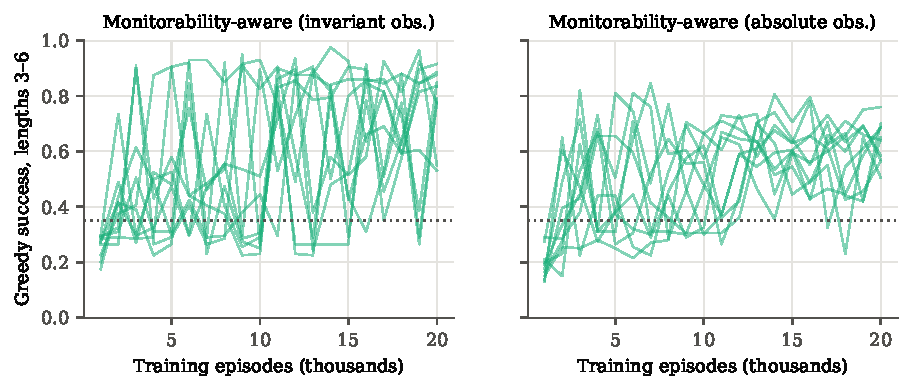
\includegraphics[width=\linewidth]{figures/policy_churn.pdf}
\caption{Greedy success on training lengths for each of the 10 seeds of the monitorability-aware agents. The dotted line marks success $0.35$. Individual runs jump between solutions throughout training; for these agents the low regime is detect-without-repair, not never-check (\S\ref{sec:norepair}).}
\label{fig:churn}
\end{figure}

\subsection{Follow-up interventions}
\label{sec:followups}

The analyses above suggest three explanations, each with a direct test. We train each intervention with the monitorability-aware reward, invariant observations and 10 seeds, and compare it with the reference agent on paired episodes (Table~\ref{tab:followups}). These comparisons are exploratory and their $p$-values are not corrected for multiplicity.

\begin{table}[t]
\centering
\small
\setlength{\tabcolsep}{3pt}
\caption{Follow-up interventions (mean over 10 seeds, 95\% $t$-interval). ``Last ckpt.'' evaluates the last checkpoint instead of the selected one; ``collapsed'' is the fraction of late checkpoints (after 5{,}000 episodes) with training-length success $\le 0.35$; ``wasted \texttt{REVISE}'' counts non-repair \texttt{REVISE}s per episode at lengths 10--14.}
\label{tab:followups}
\resizebox{\linewidth}{!}{\begin{tabular}{lcccccc}
\toprule
Variant & Success 3--6 & Success 7--9 & Success 10--14 & Last ckpt.\ 7--9 & Collapsed & Wasted REVISE \\
\midrule
Monitorability (inv) & 0.91\,{\scriptsize[0.89, 0.92]} & 0.86\,{\scriptsize[0.83, 0.89]} & 0.74\,{\scriptsize[0.68, 0.80]} & 0.63\,{\scriptsize[0.51, 0.76]} & 21\% & 0.74 \\
+ slack-per-step feature & 0.83\,{\scriptsize[0.80, 0.87]} & 0.46\,{\scriptsize[0.35, 0.57]} & 0.28\,{\scriptsize[0.20, 0.35]} & 0.37\,{\scriptsize[0.31, 0.43]} & 38\% & 0.64 \\
+ fault-located memory bit & 0.94\,{\scriptsize[0.92, 0.95]} & 0.88\,{\scriptsize[0.86, 0.91]} & 0.74\,{\scriptsize[0.65, 0.83]} & 0.81\,{\scriptsize[0.70, 0.91]} & 10\% & 0.23 \\
fault bonus paid on repair & 0.89\,{\scriptsize[0.88, 0.91]} & 0.79\,{\scriptsize[0.71, 0.87]} & 0.64\,{\scriptsize[0.52, 0.75]} & 0.75\,{\scriptsize[0.67, 0.83]} & 1\% & 0.51 \\
memory bit + bonus on repair & 0.93\,{\scriptsize[0.92, 0.95]} & 0.83\,{\scriptsize[0.76, 0.91]} & 0.66\,{\scriptsize[0.54, 0.77]} & 0.79\,{\scriptsize[0.72, 0.85]} & 0\% & 0.15 \\
+ repair-pending bit & 0.95\,{\scriptsize[0.94, 0.95]} & 0.83\,{\scriptsize[0.76, 0.91]} & 0.60\,{\scriptsize[0.45, 0.75]} & 0.89\,{\scriptsize[0.87, 0.91]} & 0\% & 0.08 \\
\bottomrule
\end{tabular}
}
\end{table}

\paragraph{Remaining-length information in unseen combinations does not help.}
Adding slack per remaining step, $\mathrm{clip}(\mathrm{slack}/(d-t), 0, 2)/2$, gives the agent the information that \S\ref{sec:residual} identifies as missing. Its values stay inside the interval seen in training, but many of them, and most of the observation vectors they form, never occur on training lengths. Observations at \val{coverage/ratio/heldout_long/unseen_rate/pct} of decision points at lengths 7--9 and \val{coverage/ratio/heldout_xlong/unseen_rate/pct} at 10--14 never appear in the training-length reference sample, against \val{coverage/invariant/heldout_long/unseen_rate/pct} and \val{coverage/invariant/heldout_xlong/unseen_rate/pct} for the invariant encoder. Held-out success falls to \val{followups/ma_ratio/heldout_long/success} at 7--9 and \val{followups/ma_ratio/heldout_xlong/success} at 10--14 ($\val{diff/ma_ratio-ma_inv/heldout_xlong/success}$, $p=\val{diff/ma_ratio-ma_inv/heldout_xlong/success/p}$). Fault detection stays high (\val{followups/ma_ratio/heldout_xlong/fault_detected}), but repairs are rarely completed (\val{followups/ma_ratio/heldout_xlong/success_given_detected}). The extra feature also hurts in distribution, by $\val{diff/ma_ratio-ma_inv/train_like/success}$ on training lengths, so its effect cannot be attributed to out-of-range inputs alone. The result is consistent with the coverage explanation, and it shows that adding the missing information is not enough.

\paragraph{A memory bit removes most wasted \texttt{REVISE}s.}
Adding one bit that records whether an \textsc{unsafe} check has been seen removes the aliasing between repairs and no-ops. Wasted \texttt{REVISE}s at 10--14 fall from \val{main/ma_inv/heldout_xlong/nonrepair_revise_count} to \val{followups/ma_memory/heldout_xlong/nonrepair_revise_count} per episode. Training-length success rises by $+$\val{diff/ma_memory-ma_inv/train_like/success} (\val{diff/ma_memory-ma_inv/train_like/success/npos}/10 seeds, $p=\val{diff/ma_memory-ma_inv/train_like/success/p}$). Held-out success at selected checkpoints does not change resolvably ($p=\val{diff/ma_memory-ma_inv/heldout_xlong/success/p}$ at 10--14), because the agent spends the recovered slack on more un-cued checks (\val{followups/ma_memory/heldout_xlong/verify_rate_cue0} vs.\ \val{main/ma_inv/heldout_xlong/verify_rate_cue0}). The allocation explanation of \S\ref{sec:residual} is therefore only partly confirmed: removing one source of waste was not enough. Checkpoint collapse is lower with the memory bit (\val{followups/ma_memory/collapse_rate/pct} vs.\ \val{main/ma_inv/collapse_rate/pct}), but the intervals overlap. The bit changes both sides of the probe. Continuing past a caught fault becomes less costly in truth (true gap \val{probe/ma_memory/true_gap}, against \val{probe/ma_inv/true_gap} without the bit), because these agents often go back and repair the fault later (a return of \val{probe/ma_memory/return_think} after continuing, against \val{probe/ma_inv/return_think}; success after continuing requires undoing back to the fault). The learned gap stays small (\val{probe/ma_memory/q_gap}).

\paragraph{Paying at the repair step removes the detect-without-repair collapse.}
Moving the $0.25$ fault bonus from detection to the first correct re-execution of the located fault places a reward at the repair step itself. If the collapse of \S\ref{sec:norepair} is a credit-assignment failure, this should help. The test changes two things at once: it removes the $0.25$ detection payment and adds a repair payment, and we do not separate them. The cue bonus is still paid when a cued fault is caught. The ablation that removes the detection payment (together with the safe-check bonus) \emph{without} adding a repair payment (no check bonuses, \S\ref{sec:ablations}) still collapses in \val{ablations/no_check_bonuses/collapse_rate/pct} [\val{ablations/no_check_bonuses/collapse_rate/lo/pct}, \val{ablations/no_check_bonuses/collapse_rate/hi/pct}] of late checkpoints. The repair payment, not the missing detection payment, is therefore the likely active ingredient. Collapsed late checkpoints drop from \val{main/ma_inv/collapse_rate/pct} [\val{main/ma_inv/collapse_rate/lo/pct}, \val{main/ma_inv/collapse_rate/hi/pct}] to \val{followups/ma_repair/collapse_rate/pct} [\val{followups/ma_repair/collapse_rate/lo/pct}, \val{followups/ma_repair/collapse_rate/hi/pct}]. The mean absolute change between consecutive evaluations drops from \val{main/ma_inv/mean_abs_change} to \val{followups/ma_repair/mean_abs_change}. With the memory bit added as well, collapse disappears entirely (\val{followups/ma_memory_repair/collapse_rate/pct}). The repair payment widens the learned gap between repairing and continuing after a caught fault, from \val{probe/ma_inv/q_gap} to \val{probe/ma_repair/q_gap}, and to \val{probe/ma_memory_repair/q_gap} with the memory bit (medians over \textsc{unsafe} decision points). The true gaps are about two (\val{probe/ma_inv/true_gap}, \val{probe/ma_repair/true_gap} and \val{probe/ma_memory_repair/true_gap}), so even the larger learned gaps are far too small, but they appear large enough to keep the greedy choice stable.

The benefit shows up in \emph{reliability} rather than peak performance. At selected checkpoints the repair-paid reward does not beat the original, because selection already discards collapsed checkpoints. It may even be slightly worse there: \val{diff/ma_repair-ma_inv/heldout_long/success} [\val{diff/ma_repair-ma_inv/heldout_long/success/lo}, \val{diff/ma_repair-ma_inv/heldout_long/success/hi}] at 7--9 ($p=\val{diff/ma_repair-ma_inv/heldout_long/success/p}$) and \val{diff/ma_repair-ma_inv/heldout_xlong/success} [\val{diff/ma_repair-ma_inv/heldout_xlong/success/lo}, \val{diff/ma_repair-ma_inv/heldout_xlong/success/hi}] at 10--14, differences that 10 seeds do not resolve. At the last checkpoint it is better: $+$\val{diff/ma_repair@final-ma_inv@final/heldout_long/success} [\val{diff/ma_repair@final-ma_inv@final/heldout_long/success/lo}, \val{diff/ma_repair@final-ma_inv@final/heldout_long/success/hi}] at 7--9 ($p=\val{diff/ma_repair@final-ma_inv@final/heldout_long/success/p}$) and $+$\val{diff/ma_repair@final-ma_inv@final/heldout_xlong/success} at 10--14 ($p=\val{diff/ma_repair@final-ma_inv@final/heldout_xlong/success/p}$).

The two last-checkpoint agents behave differently. The repair-paid agent checks less (\val{followups/ma_repair@final/heldout_long/verify_count} vs.\ \val{main/ma_inv@final/heldout_long/verify_count} checks per episode) and catches fewer faults (\val{followups/ma_repair@final/heldout_long/fault_detected} vs.\ \val{main/ma_inv@final/heldout_long/fault_detected}). But it almost always completes the repairs it starts (\val{followups/ma_repair@final/heldout_long/success_given_detected} vs.\ \val{main/ma_inv@final/heldout_long/success_given_detected}).

